\chapter{Teória strojového učenia I}

Chceme sa naučiť na základe nejakých vstupných dát $x$ predikovať $y$.
Môžeme si to predstaviť tak, že príroda vie poskytovať pozorovania,
každé v tvare dvojice $(x, y)$. Dostali sme od nej sadu $t$ pozorovaní,
na základe ktorých chceme navrhnúť nejakú funkciu $h$, ktorá predpovedá
$y$ na základe $x$. Dobrá funkcia je taká, ktorá je schopná
\emph{zovšeobecňovať}, teda sa jej ``dobré darí'' aj na dátach mimo
trénovacej množiny. Proces, ktorým $h$ zostrojíme, si môžeme predtaviť
ako algoritmus, ktorý berie ako vstupy trénovacie dáta a vráti nám
funkciu.




\section{Matematický model}

Z matematického hľadiska, prírodu vieme formalizovať ako
pravdepodobnostnú distribúciu $P$. Množinu všetkých možných
$x$ označíme $X$, množinu možných $y$ označíme $Y$.

V tejto časti sa nebudeme zaoberať výpočtovou stránkou strojového
učenia, od detailov ako časová zložitosť, ..., abstrahujeme. Algoritmus
si teda predstavíme iba ako niečo, čo vezme ako vstup trénovacie dáta
$(x_1, y_1), \ldots, (x_t, y_t)$ a na výstup vráti funkciu
$h : X \to Y$. Túto funkciu budeme volať \emph{hypotéza}. Množinu
všetkých možných funkcii, ktoré môže náš algoritmus vrátiť,
budeme volať \emph{množina hypotéz} a značiť ho $H$.

\paragraph{Chyba hypotézy.}
Ako vyjadriť mieru toho, že sa funkcii ``dobre darí''? Spravíme tak
pomocou \emph{chybovej funkcie} $\err : Y \times Y \to \reals^+$,
ktorej význam je nasledovný: $\err(y, y')$ vyjadruje, ako veľmi
sa od seba líšia $y$ a $y'$. Pomocou tejto funkcie vieme odmerať
priemernú chybu hypotézy $h$, ktorú budeme tiež označovať $\err$,
nasledovne:
$$\err(h) = \E_{x, y} \left[ \err(h(x), y) \right]$$
Pod $\E_{x, y}$ sa rozumie stredná hodnota cez $(x, y)$
z pravdepodobnostnej distribúcie $P$, teda $(x, y) \sim P$.
Pri klasifikácii sa zvykne používať chybová funkcia
$$
  \err(y, y') = \left\{
    \begin{array}{ll}
      0, & \text{ak}\ y = y' \\
      1, & \text{inak}
    \end{array}
  \right.
$$
a potom zrejme
$$\E_{x, y} \left[ \err(h(x), y) \right] = \prob_{x, y} \left( h(x) \neq y \right).$$
Pri regresii máme viacero možností, bežné voľby sú kvadratická chyba
$(y - y')^2$ a absolútna chyba $|y - y'|$.

\paragraph{Chyba algoritmu.}
Ako vyjadriť chybu celého učiaceho algoritmu? Uvedomme si, že výstup
algoritmu je závislý od trénovacích dát $T = \{(x_1, y_1), \ldots, (x_t, y_t)\}$,
ktoré dostane. Takže výstupná funkcia je od nich závislá, budeme ju
označovať $\hat{h}$. Potom priemerná chyba algoritmu (alebo inak
\emph{priemerná chyba priemernej hypotézy}), braná cez všetky možné
vzorky trénovacích dát, je rovná
$$\E_T \left[ \err(\hat{h}) \right] = \E_T \left[ \E_{x,y} \left[ \err(\hat{h}(x), y) \right] \right].$$
Pod $\E_T$ sa rozumie stredná hodnota cez všetky možné $t$-tice
trénovacích dát $T$, brané nezávisle z pravdepodobnostnej
distribúcie $P$.

\paragraph{Trénovacia chyba.}
Pri vyššie uvedených chybách sme vždy merali vzhľadom na skutočnú
distribúciu $P$. Môže nás ale zaujímať, aká je priemerná chyba
hypotézy na trénovacích dátach $T$. Túto chybu budeme označovať
$\err_T(h)$, a vypočítame ju ako
$$\err_T(h) = \E_{x_i, y_i} \left[ \err(h(x_i), y_i) \right] = \frac{1}{t} \cdot \sum_{i=1}^t \err(h(x_i), y_i).$$

Priemerná trénovacia chyba z pohľadu algoritmu bude
$$\E_T \left[ \err_T(\hat{h}) \right].$$

V nasledujúcom texte budeme vynechávať premenné, cez ktoré prebiehajú
stredné hodnoty, všade tam, kde budú zrejmé z kontextu.




\section{Analýza veľkostí chýb}

V tejto časti sa podrobnejšie pozrieme na to, ako závisia vyššie
uvedené štatistiky (tj. priemerná testovacia a trénovacia chyba
priemernej hypotézy) od veľkosti trénovacej množiny $T$ a od veľkosti
množiny hypotéz $H$.

V celej časti budeme predpokladať, že úloha je regresného
charakteru a chyba sa meria ako kvadratická odchýlka, teda
$$\err(y, y') = (y - y')^2.$$



\subsection{Teoretické limity}
Najprv sa ale pozrieme na teoretické limity toho, ako dobrá vôbec
môže nejaká funkcia byť. Označme $h^{\square}$ najlepšiu možnú funkciu,
nemusí byť nutne z $H$. Teda
$$h^{\square} = \argmin_h \left( \err(h) \right) = \argmin_h \left( \E_{x,y} \left[ (h(x) - y)^2 \right] \right).$$
Jediné obmedzenia kladené na $h$ sú, že je to funkcia: pre každé $x$
musí vrátiť vždy jednu a tú istú hodnotu. Distribúcia $P$ ale nemusí
pre dané $x$ vždy vrátiť to isté $y$: môže byť zašumená, alebo
jednoducho $x$ neobsahuje dostatočnú informáciu. Napríklad, ak podľa
plochy bytu určujeme jeho cenu, niektoré dva byty môžu mať rovnakú
plochu a predsa rôznu cenu. Ako uvidíme, tento nedeterminizmus je
jediný dôvod, prečo hypotéza $h^{\square}$ nemusí mať nulovú chybu.

Chybu ľubovoľnej hypotézy $h$ vieme upraviť nasledovne:
\begin{align}
  \err(h)
    &= \E_{x,y} \left[ (h(x) - y)^2 \right] \\
    &= \E_{x} \left[ \E_{y|x} \left[ (h(x) - y)^2 \right] \right]
\end{align}
Pozrime sa na vnútornú strednú hodnotu. V nej je $x$ konštanta, a
teda aj $h(x) = c$ je konštanta. Aká konštanta minimalizuje danú
strednú hodnotu? Nie je ťažké vidieť (napríklad zderivovaním), že
minimum sa nadobúda pre $c = \E[y]$. Takže
$$h^{\square}(x) = \E_{y|x}[y],$$
a jeho priemerná chyba je
$$\err(h^{\square}) = \E_{x} \left[ \E_{y|x} \left[ (y - \E[y]) \right] \right] = \E_{x} \left[ \Var_{y|x}(y) \right].$$
Vidíme teda, že pokiaľ je $y$ jednoznačne určené $x$-om, tak
$h^{\square}$ bude mať nulovú chybu.



\subsection{Bias-variance tradeoff}
V tomto odseku si ukážeme zaujímavý výsledok, ktorý nám za určitých
predpokladov umožňuje vyjadriť chyby pomocou iných, jasnejších veličín:
tzv. \emph{výchylky} a \emph{rozptylu}.
Označme najlepšiu hypotézu z množiny $H$ ako $h^\star$, teda
$$h^\star = \argmin_h \left( \err(h) \right).$$

Budeme upravovať výraz reprezentujúci priemernú chybu priemernej
hypotézy $\hat{h}$.
\begin{align}
  \chalg % \E_T \left[ \err(\hat{h}) \right]
    &= \E_T \left[ \err(\hat{h}) \right] \\
    &= \E_T \left[ \E_{x,y} \left[ (\hat{h}(x) - y)^2 \right] \right] \\
    &= \E_T \left[ \E_{x,y} \left[ \left( (\hat{h}(x) - h^\star(x)) + (h^\star(x) - y) \right)^2 \right] \right]
\end{align}
V tomto momente prichádza netriviálny technický krok, ktorý si
vyžaduje dodatočné predpoklady. Tieto technické detaily prenecháme
na koniec časti, sústreďme sa na to hlavné.
$$
  \chalg
    = \E_T \left[ \E_{x,y} \left[ (\hat{h}(x) - h^\star(x))^2 \right] \right]
    + \E_T \left[ \E_{x,y} \left[ (h^\star(x) - y)^2 \right] \right]
$$
Druhý zo sčítancov sa dá ešte zjednodušiť. Kedže $h^\star$ ani $y$
nezávisia od trénovacích dát, môžeme sa zbaviť vonkajšej strednej
hodnoty. Dostávame tak výslednú rovnosť
$$
  \chalg
    = \underbrace{\E_T \left[ \E_{x,y} \left[ (\hat{h}(x) - h^\star(x))^2 \right] \right]}_{\text{rozptyl}}
    + \underbrace{\E_{x,y} \left[ (h^\star(x) - y)^2 \right]}_{\text{výchylka}}.
$$

Prvý zo sčítancov budeme volať \emph{rozptyl}. Trénovací algoritmus
s malým rozptylom vracia funkcie, ktoré sú blízko optima v množine $H$.
Tým, že mu zväčšíme množinu trénovacích dát, si veľmi neprilepšíme.
Naopak, algoritmus s veľkým rozptylom vracia funkcie ďaleko od optima,
teoreticky by sme sa teda vedeli k optimu priblížiť tým, že zväčšíme
množstvo trénovacích dát.

\medskip

Druhý zo sčítancov budeme volať \emph{výchylka}. Vyjadruje chybu, ktorá
je spôsobená tým, že sa náš algoritmus obmedzil na nejakú konkrétnu
množinu hypotéz $H$. Čím väčšia množina hypotéz, tým menšia výchylka
(nakoľko $h^\star$ je najlepšia hypotéza v množine $H$, jej zväčšením
si môžeme iba prilepšiť). Zložitejšia množina hypotéz ale ľahšie
``napasuje'' na ľubovoľné trénovacie dáta. To zvyšuje riziko toho,
že výsledná hypotéza bude špecifická pre obdržané dáta, a nebude
schopná zovšeobecňovať mimo nich. Je teda potreba väčšieho množstva
trénovacích dát.

\medskip

Ak máme fixné trénovacie dáta $T$, pri voľbe množiny hypotéz $H$ sa snažíme
nájsť kompromis medzi malým rozptylom a malou výchylkou. Zložité $H$
bude mať malú výchylku ale veľký rozptyl, čo vedie k tzv. \emph{preučeniu}.
Jednoduché $H$ bude mať malý rozptyl, ale veľkú výchylku, tzv. \emph{podučenie}.

Na obrázku \ref{img:fitting} ilustrujeme oba koncepty: úlohou je modelovať
kvadratickú funkciu. Ak za množinu hypotéz zvolíme lineárne funkcie,
ich chyby sa nebudú veľmi od seba líšiť, ale všetky budú zle. Ak za
množinu hypotéz zvolíme polynómy nejakého vysokého stupňa, ľahko
nájdeme polynóm prechádzajúci cez trénovacie dáta, avšak mimo nich
bude dávať výsledky úplne mimo.

\begin{figure}
  \centering
  \begin{subfigure}[b]{0.3\linewidth}
    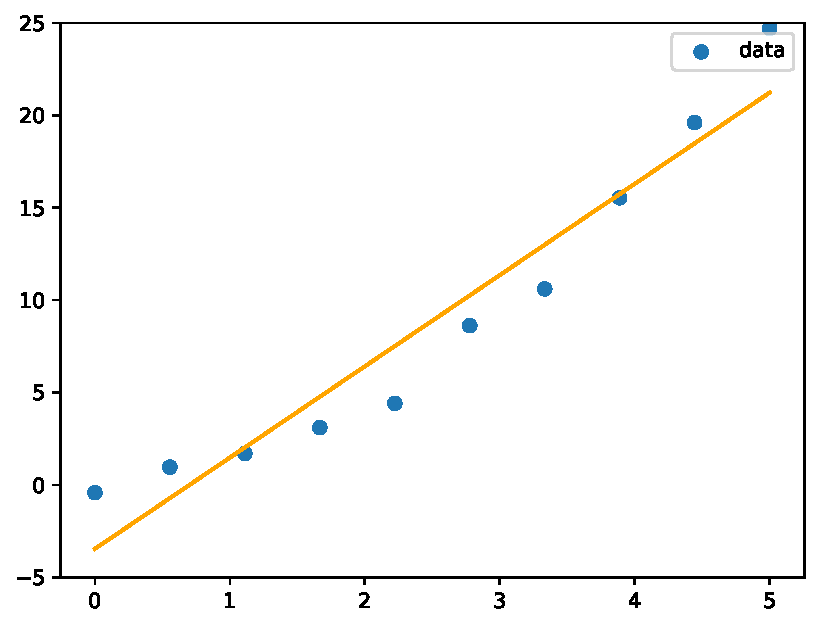
\includegraphics[width=\linewidth]{obrazky/fitting1.pdf}
  \end{subfigure}
  ~
  \begin{subfigure}[b]{0.3\textwidth}
    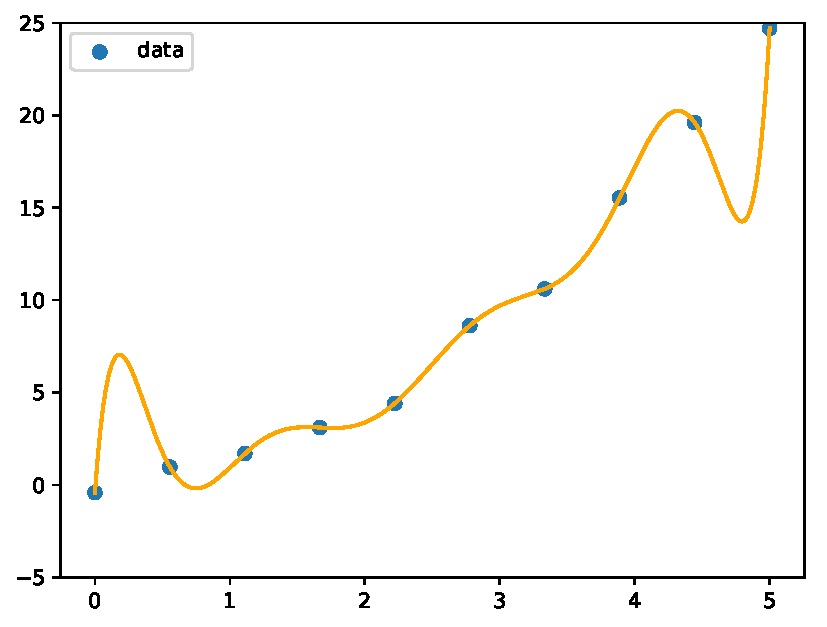
\includegraphics[width=\linewidth]{obrazky/fitting9.pdf}
  \end{subfigure}
  ~
  \begin{subfigure}[b]{0.3\textwidth}
    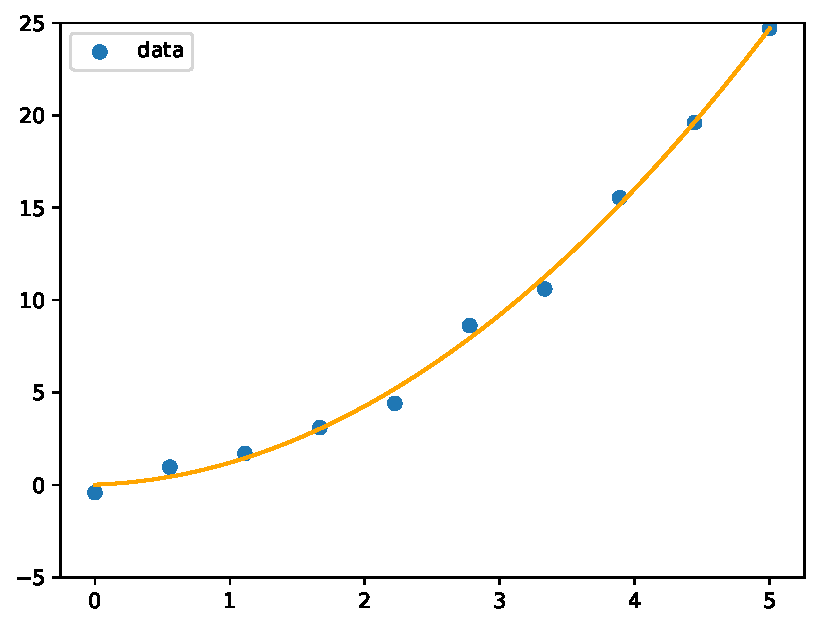
\includegraphics[width=\linewidth]{obrazky/fitting2.pdf}
  \end{subfigure}
  \caption{Podučenie, preučenie, akurát.}
  \label{img:fitting}
\end{figure}

\medskip

Výchylku vieme upraviť ďalej. Hypotéza $h^\star$ ani $y$ nezávisia
od trénovacej množiny $T$. Z ich pohľadu sú teda testovacie dáta $x, y$
a trénovacie dáta $x_i, y_i$ nerozoznateľné. Takže na meranie chyby
$h^\star$ môžeme použiť trénovacie dáta (berúc v úvahu ich náhodný
výber):
\begin{align}
  \vychylka
    &= \E_T \left[ \E_{x_i, y_i} \left[ (h^\star(x_i) - y_i)^2 \right] \right] \\
    &= \E_T \left[ \E_{x_i, y_i} \left[ \left( (h^\star(x_i) - \hat{h}(x_i)) + (\hat{h}(x_i) - y_i) \right)^2 \right] \right]
\end{align}
Použitím ďalšieho technického kroku dostaneme:
\begin{align}
  \vychylka &= \underbrace{\E_T \left[ \E_{x_i, y_i} \left[ (h^\star(x_i) - \hat{h}(x_i))^2 \right] \right]}_{\text{trénovací rozptyl}}
    + \underbrace{\E_T \left[ \E_{x_i, y_i} \left[ (\hat{h}(x_i) - y_i)^2 \right] \right]}_{\text{priemerná trénovacia chyba}}
\end{align}

Prvý zo sčítancov budeme volať \emph{trénovací rozptyl}.
Uvedomme si, že pre ľubovoľné trénovacie dáta $T$ platí
$$\err_T(\hat{h}) \leq \err_T(h^\star),$$
nakoľko $\hat{h}$ je optimálna hypotéza pre danú množinu trénovacích
dát. Hypotéza $h$ síce je najlepšia pre $H$, trénovacie dáta sú ale len
malá vzorka z $H$.
Trénovací rozptyl teda môžeme chápať ako mieru toho, ako veľmi
reprezentatívnu vzorku trénovacích dát sme dostali. Čím menší je,
tým viac reprezentatívna vzorka je.

\medskip

Druhý zo sčítancov budeme volať \emph{priemerná trénovacia chyba}.
Je to priemerná chyba, ktorej sa dopustí výstu z algoritmu $\hat{h}$
na tých istých dátach, pomocou ktorých sme $\hat{h}$ zostrojili.

\medskip

Platí
$$ {\normalfont \text{priemerná trénovacia chyba}} \leq \vychylka \leq \chalg. $$
Na konkrétnych trénovacích dátach ale nemusí platiť, že trénovacia
chyba je menšia ako testovacia chyba: mohli sme si (síce s malou
pravdepodobnosťou, ale predsa) vytiahnuť zlé trénovacie dáta, ktoré
sa výrazne líšia od skutočných dát.

\medskip

Na základe dosiaľ uvedeného vieme graficky znázorniť, ako sa zhruba správajú
rozptyl, výchylka, trénovací rozptyl a priemerná trénovacia chyba,
v závislosti od veľkosti trénovacej množiny (obrázok \ref{img:train})
a od zložitosti množiny hypotéz (obrázok \ref{img:hypo}).


\TODO{obrázok kriviek učenia, vysvetlenie}


\paragraph{Technické detaily.}
Nakoniec sa vyjadríme k spomínanému technickému kroku. Začneme jeho
znením a potom uvedieme jeho predpoklady.

\begin{theorem} \label{theorem:proj1}
  Predpokladajme, že vstupom do hypotéz sú vektory reálnych čísel
  (tj. $X = \reals^n$), cieľom je predpovedať jedno reálne číslo
  (tj. $Y = \reals$), a že pravdepodobnostné rozdelenie $P$ je spojité.
  
  Nech množina hypotéz $H$ je uzavretá na lineárne kombinácie a na
  limity (teda ak postupnosť funkcii v $H$ konverguje, jej limita
  je tiež v $H$).
  
  Ďalej predpokladajme, že trénovací algoritmus vždy vráti takú funkciu
  $\hat{h} \in H$, ktorá minimalizuje trénovaciu chybu. Inak zapísané,
  $$\hat{h} = \argmin_{h \in H} \left( \E_T \left[ \err_T(h) \right] \right).$$
  
  Potom platí
  $$\E_T \left[ \E_{x,y} \left[ \left( (\hat{h}(x) - h^\star(x)) + (h^\star(x) - y) \right)^2 \right] \right] = \E_T \left[ \E_{x,y} \left[ (\hat{h}(x) - h^\star(x))^2 \right] \right] + \E_T \left[ \E_{x,y} \left[ (h^\star(x) - y)^2 \right] \right]$$
\end{theorem}
\begin{remark}
  Dokazovaná rovnosť je ekvivalentná s nasledovnou, stručnejšou:
  $$\E_T \left[ \E_{x, y} \left[ (\hat{h}(x) - h^\star(x)) \cdot (h^\star(x) - y) \right] \right] = 0.$$
  Túto kratšiu verziu získame roznásobením a použitím linearity strednej
  hodnoty. V dôkaze budeme dokazovať túto rovnosť.
\end{remark}
\begin{remark}
  Všimnite si, že potrebujeme uzavretosť množiny $H$ na limity na to,
  aby vôbec $\argmin_{h \in H} (\ldots)$ existovalo. Vo všeobecnosti
  nemusí existovať taká funkcia, ale môže existovať nekonečná postupnosť
  funkcii, každá ďalšia lepšia, ako tá predchádzajúca. (Inak povedané,
  neexistuje minimum, iba infimum.)
\end{remark}
\begin{remark}
  Je namieste otázka, či je $\argmin_{h \in H} (\ldots)$ dobre definované,
  teda či je taká funkcia $h$ práve jedna. Za chvíľu uvidíme, že naše
  predpoklady to zaručujú.
\end{remark}
\begin{remark}
  Veta by sa dala rozšíriť aj na iné množiny $X, Y$, napríklad keď
  predpovedaná premenná je vektor ($Y = \reals^m$), ... Možno ani $P$
  nemusí byť spojité. Pre jednoduchosť argumentu ale budeme uvažovať
  vetu tak, ako je popísaná vyššie.
\end{remark}
\begin{remark}
  Predpoklady vety sú značne obmedzujúce. Napríklad si uvedomte, že
  ju nie je možné použiť na klasifikáciu, či dokonca ani na ľubovoľnú
  ohraničenú regresiu (kde rozumné hodnoty $y$ sú ohraničené). Ale taká
  je teória.
\end{remark}

Pri našom dôkaze využijeme niekoľko vlastností funkcii, ktoré uvádzame
v nasledujúcom odseku. Skúsený čitateľ-matematik ho môže preskočiť.

\begin{definition}
  (Skalárny súčin.) Nech $f, g$ sú funkcie z $X$ do $\reals$,
  z nejakej príjemne sa správajúcej množiny funkcii (tj. rovnomerne
  spojité, ..., čokoľvek, aby nasledujúce argumenty prešli). Definujeme
  ich skalárny súčin $\langle \cdot, \cdot \rangle$ ako
  \begin{align}
    \langle f, g \rangle
      &= \int f(x) \cdot g(x)\ d\rho x \\
      &= \E_x \left[ f(x) \cdot g(x) \right],
  \end{align}
  kde $\rho$ je hustota pravdepodobnosti distribúcie $P$.
  Rozmyslite si, že takto definovaný skalárny súčin má všetky vlastnosti,
  ktoré sa bežne požadujú od skalárnych súčinov:
  \begin{itemize}
    \item Je symetrický od svojich argumentov, teda $\langle f, g \rangle = \langle g, f \rangle$.
    \item Je lineárny: $\langle f, g + h \rangle = \langle f, g \rangle + \langle f, h \rangle$
      a tiež $\langle k \cdot f, g \rangle = k \cdot \langle f, g \rangle$.
    \item $\langle f, f \rangle \geq 0$ pre ľubovoľné $f$, pričom rovnosť
      nastáva práve vtedy, keď je $f$ konštantne nulové.
  \end{itemize}
\end{definition}

\begin{definition}
  (Kolmosť.) Dve funkcie $f, g$ sú na seba kolmé, ak ich skalárny
  súčin je $0$. Značíme $f \perp g$.
\end{definition}

\begin{definition}
  (Norma.) Podľa skalárneho súčinu definujeme normu funkcie (jej ``dĺžku''):
  $$\norm{f} = \sqrt{\langle f, f \rangle} = \sqrt{\E_x \left[ f^2(x) \right] }$$
  Spĺňa \emph{trojuholníkovú nerovnosť}: pre ľubovoľné funkcie $f, g$
  platí
  $$\norm{f} + \norm{g} \geq \norm{f + g}.$$
  Definuje nám teda (euklidovskú) metriku nad funkciami, podľa
  ktorej definujeme limity a konvergenciu.
\end{definition}

\begin{lemma}
  (Pytagorova veta.) Nech $f \perp g$. Potom platí:
  $$\norm{f}^2 + \norm{g}^2 = \norm{f + g}^2$$
\end{lemma}
\begin{proof}
  Pozrime sa na pravú stranu. Iba v nej zapíšeme normu ako skalárny
  súčin a využijeme jeho linearitu a symetriu:
  \begin{align}
    \norm{f + g}^2
      &= \langle f + g, f + g \rangle \\
      &= \langle f, f \rangle + \langle g, g \rangle + 2 \cdot \langle f, g \rangle
  \end{align}
  Pretože $f \perp g$, posledný sčítanec je nulový, čím dostávame
  dokazované tvrdenie.
\end{proof}

\begin{definition}
  (Projekcia na množinu.) \emph{Projekciu} funkcie $f$ na množinu $H$
  budeme označovať $f_H$ a budeme pod ňou rozumieť nasledovný výraz:
  $$f_H = \argmin_{h \in H} d(f, h)$$
\end{definition}

\begin{remark}
  Ako sa už spomínalo, nie je zrejmé, že projekcia je dobre definovaná.
  Preto v nasledujúcej lemme definujeme $f_H$ trochu iným spôsobom, ako
  jednu z možno viacerých funkcii, ktoré minimalizujú vzdialenosť k $H$.
\end{remark}

\begin{lemma} \label{lem:projperp}
  (Kolmosť projekcie.) Pre ľubovoľnú funkciu $h \in H$ platí $h \perp f - f_H$.
\end{lemma}
\begin{proof}
  Sporom, predpokladajme, že $h \not\perp f - f_H$. Takže
  $\langle h, f - f_H \rangle \neq 0$. Ukážeme, že potom existuje
  v $H$ funkcia, ktorá je k funkcii $f$ bližšie, ako funkcia $f_H$.
  To bude hľadaný spor s definíciou $f_H$.
  
  Pozrime sa na všetky funkcie, ktoré ležia na priamke
  $f_H + \Delta \cdot h$. Tieto funkci sú v množine $H$, pretože
  $f_H, h \in H$ a množina $H$ je uzavretá na lineárne kombinácie.
  Každú z týchto funkcii vieme asociovať s jedným reálnym číslom
  $\Delta$. Pozrime sa na ich vzdialenosti od funkcie $f$, vyjadrené
  ako funkcia od $\Delta$:
  \begin{align}
    \text{dist}(\Delta)
      &= d(f, f_H + \Delta \cdot h) \\
      &= \langle (f - f_H) + \Delta \cdot h, (f - f_H) + \Delta \cdot h \rangle \\
      &= \langle f - f_H, f - f_H \rangle + 2\Delta \cdot \langle h, f - f_H \rangle + \Delta^2 \cdot \langle h, h \rangle
  \end{align}
  Pozrime sa na deriváciu tejto funkcie. Podľa definície $f_H$ by
  malo byť $f - f_H$ najkratšie možné, teda pre $\Delta = 0$ by mala
  funkcia $\text{dist}$ nadobúdať minimum, a teda mať tam nulovú
  deriváciu. Uvidíme, že tomu tak nie je:
  \begin{align}
    \frac{\partial \text{dist}}{\partial \Delta} \left( 0 \right)
      &= \lim_{\Delta \to 0} \left( \frac{\text{dist}(\Delta) - \text{dist}(0)}{\Delta} \right) \\
      &= \lim_{\Delta \to 0} \left( \frac{2\Delta \cdot \langle h, f - f_H \rangle + \Delta^2 \cdot \langle h, h \rangle}{\Delta} \right) \\
      &= 2 \cdot \langle h, f - f_H \rangle
  \end{align}
  To je nenulové, nakoľko $h \not \perp f - f_H$. Čo je hľadaný spor.
\end{proof}

\begin{lemma}
  Projekcia na množinu $H$ je dobre definovaná, teda vždy existuje
  nanajvýš jedna funkcia $f_H \in H$, ktorá minimalizuje vzdialenosť
  k $f$.
\end{lemma}
\begin{proof}
  Predpokladajme, že také funkcie sú dve, označme ich $g, h$. Ukážeme,
  že potom nutne $g = h$.
  
  Podľa predchádzajúcej lemmy platí
  \begin{align}
    f - g \perp g,\ \text{odkiaľ} &\langle f - g, g \rangle = 0 \\
                                  &\langle f - h, g \rangle = 0 \\
                                  &\langle f - g, h \rangle = 0 \\
                                  &\langle f - h, h \rangle = 0
  \end{align}
  Z týchto rovností dostaneme
  $$\langle g, g \rangle = \langle g, h \rangle = \langle h, g \rangle = \langle h, h \rangle.$$
  Nakoniec, pozrime sa na normu funkcie $g - h$:
  \begin{align}
    \norm{g - h}
      &= \sqrt{\langle g - h, g - h \rangle} \\
      &= \sqrt{\langle g, g \rangle - \langle g, h \rangle - \langle h, g \rangle + \langle h, h \rangle} \\
      &= 0
  \end{align}
  To môže nastať jedine vtedy, keď $g = h$.
\end{proof}

\begin{lemma} \label{lem:hsq}
  Hypotéza $h^\star$ je projekciou $h^\square$ na $H$, teda $h^\star = h^\square_H$.
\end{lemma}
\begin{proof}
  Vychádzajme z definície $h^\star$.
  \begin{align}
    h^\star
      &= \argmin_{h \in H} \E_{x,y} \left[ (h(x) - y)^2 \right] \\
      &= \argmin_{h \in H} \E_{x,y} \left[ \left( (h(x) - h^\square(x)) + (h^\square(x) - y) \right)^2 \right] \\
      &= \argmin_{h \in H} \left(
        \begin{array}{ll}
          &\E_{x,y} \left[ (h(x) - h^\square(x))^2 \right] \\
          + &\E_{x,y} \left[ (h^\square(x) - y)^2 \right] \\
          + 2 \cdot &\E_{x,y} \left[ (h(x) - h^\square(x)) \cdot (h^\square(x) - y) \right]
        \end{array}
        \right)
  \end{align}
  Druhý sčítanec je konštanta, teda nám $\argmin$ nijak neovplyvňuje.
  Tretí sčítanec vieme upraviť nasledovne:
  \begin{align}
    \text{tretí sčítanec}
      &= \E_x \left[ \E_{y|x} \left[ (h(x) - h^\square(x)) \cdot (h^\square(x) - y) \right] \right] \\
      &= \E_x \left[ (h(x) - h^\square(x)) \cdot \E_{y|x} \left[ h^\square(x) - y \right] \right] \\
      &= 0
  \end{align}
  A teda je to tiež konštanta. Dostávame tak
  $$h^\star = \argmin_{h \in H} \E_{x,y} \left[ (h(x) - h^\square(x))^2 \right],$$
  čo je presne definícia projekcie $h^\square$ na množinu $H$.
\end{proof}

Vyzbrojení týmito znalosťami, môžeme sa vrhnúť na dôkaz vety \ref{theorem:proj1}.
Pripomeňme si ešte pred tým dokazovanú rovnosť:
$$\E_T \left[ \E_{x, y} \left[ (\hat{h}(x) - h^\star(x)) \cdot (h^\star(x) - y) \right] \right] = 0.$$

\begin{proof}
  Ľavú stranu dokazovanej rovnosti vieme prepísať do nasledovného,
  ekvivalentného tvaru:
  $$ = \E_T \left[ \E_{x, y} \left[ (\hat{h}(x) - h^\star(x)) \cdot ((h^\star(x) - h^\square(x)) + (h^\square(x) - y)) \right] \right] $$
  Vieme, že $\varepsilon := h^\square(x) - y$ sa správa pre dané $x$
  ako náhodná premenná, ktorá má strednú hodnotu $0$ a je nezávislá
  od ostatných premenných vystupujúcich vo výraze. Z výrazu ju teda
  môžeme vyhodiť, dostaneme tak
  $$ = \E_T \left[ \E_{x, y} \left[ (\hat{h}(x) - h^\star(x)) \cdot (h^\star(x) - h^\square(x)) \right] \right] $$
  Stačí nám teda dokázať $\hat{h} - h^\star \perp h^\star - h^\square$.
  To ale vyplýva z lemmy o kolmosti projekcie (\ref{lem:projperp}).
  Overíme, že jej podmienky sú splnené: z uzavretosti na lineárne
  kombinácie platí $\hat{h} - h^\star \in H$, a podľa lemmy \ref{lem:hsq}
  platí $h^\star = h^\square_H$, odkiaľ
  $h^\star - h^\square = -(h^\square - h^\square_H)$.
  Záporné znamienko na kolmosti nič nemení.
\end{proof}

Podobným spôsobom sa dá dokázať aj korektnosť druhého technického
kroku. To prenechávame čitateľovi ako cvičenie.



\subsection{Bias-variance tradeoff, verzia 2.}
V literatúre pod názvom \emph{bias-variance tradeoff} vystupuje aj
podobný, ale predsa odlišný výsledok, ako bolo uvedené vyššie.
Ukážeme a odvodíme si ho.

\begin{theorem}
  Nech $y : X \to \reals$ je funkcia, ktorú sa snažíme modelovať.
  Predpokladajme, že sa dá rozložiť na časti: $y = f(x) + \varepsilon$,
  kde $\varepsilon$ hrá rolu šumu: je nezávislý od všetkého a
  $\E[\varepsilon] = 0$. Označíme jeho pravdepodobnostnú distribúciu
  $E$.
  
  Nech výstupom trénovacieho algoritmu je $\hat{f}$. Za chybovú
  funkciu zvoľme kvadratickú chybu. Chybu algoritmu vieme teda
  vypočítať nasledovne:
  $$\chalg = \E_{(x, y) \sim P, T \sim P^t, \varepsilon \sim E} \left[ (\hat{f}(x) - y)^2 \right].$$
  
  Tvrdíme, že sa dá rozložiť na tri nasledovné časti:
  $$
  \chalg
      = \underbrace{\Var(\hat{f}(x) - f(x))}_{\text{\normalfont rozptyl}}
      + \underbrace{(\E[\hat{f}(x)] - \E[f(x)])^2}_{\text{\normalfont výchylka}^2}
      + \underbrace{\Var(\varepsilon)}_{\text{\normalfont šum}}
  $$
\end{theorem}
\begin{remark}
  V poslednej rovnici sme kvôli stručnosti vynechali pri stredných
  hodnotách a rozptyloch premenné a distribúcie, z ktorých ich berieme.
  V dôkaze budeme vždy brať všetky premenné z ich príslušných distribúcii.
\end{remark}
\begin{remark}
  Funkcia $f$ hrá v podstate tú istú rolu, čo najlepšia možná hypotéza
  spomedzi všetkých funkcii (nielen tých v množine hypotéz), $h^\square$.
\end{remark}
\begin{remark}
  V tomto znení bias-variance tradeoff-u názvy \emph{rozptyl} a
  \emph{výchylka} zodpovedajú príslušným štatistickým/pravdepodobnostným
  pojmom.
\end{remark}
\begin{remark}
  Na rozdiel od predchádzajúcej verzie bias-variance tradeoff-u, tu
  nebudeme potrebovať žiadne dodatočné predpoklady od algoritmu ani
  od jeho množiny hypotéz. (Nemusí teda vracať hypotézu, ktorá je
  spomedzi hypotéz v $H$ najlepšia na daných trénovacích dátach.
  Takisto od množiny hypotéz nepožadujeme žiadne vlastnosti.)
\end{remark}
\begin{proof}
  Upravujme pôvodný výraz.
  \begin{align}
    \chalg
      &= \E \left[ (\hat{f}(x) - y)^2 \right] \\
      &= \E \left[ (\hat{f}(x) - f(x) - \varepsilon)^2 \right] \\
      &= \E \left[ (\hat{f}(x) - f(x))^2 \right] + \E \left[ \varepsilon^2 \right] - 2 \cdot \E \left[ \varepsilon \cdot (\hat{f}(x) - f(x)) \right] \\
      &= \E \left[ (\hat{f}(x) - f(x))^2 \right] + \E \left[ \varepsilon^2 \right]
  \end{align}
  Výraz sme upravili, roznásobili a využili linearitu strednej hodnoty.
  V poslednom kroku sme použili $\E[ab] = \E[a] \cdot \E[b]$, ktorý
  platí pre ľubovoľné nezávislé premenné, s $a := \varepsilon$,
  $b := \hat{f}(x) - f(x)$. Zamerajme sa ďalej na prvý sčítanec.
  \begin{align}
    \text{prvý sčítanec}
      &= \E \left[ (\hat{f}(x) - f(x))^2 \right] \\
      &= \E[\hat{f}(x)^2] + \E[f(x)^2] - 2 \cdot \E[\hat{f}(x) \cdot f(x)] \\
      &= (\Var(\hat{f}(x)) + \E[\hat{f}(x)]^2) + (\Var(f(x)) + \E[f(x)]^2) - 2 \cdot \E[\hat{f}(x) \cdot f(x)]
  \end{align}
  V poslednom kroku sme využili vzťah $\Var(a) = \E[a^2] - \E[a]^2$.
  Pokračujme ďalej v úpravách.
  \begin{align}
    \begin{split}
      \text{prvý sčítanec}
        &= \Var(\hat{f}(x)) + \Var(f(x)) + (\E[\hat{f}(x)] - \E[f(x)])^2 \\
        &\quad + 2 \cdot \E[\hat{f}(x)] \cdot \E[f(x)] - 2 \cdot \E[\hat{f}(x) \cdot f(x)]
    \end{split} \\
    &= \Var(\hat{f}(x)) + \Var(f(x)) + (\E[\hat{f}(x)] - \E[f(x)])^2 - 2 \cdot \Cov(\hat{f}(x), f(x)) \\
    &= \Var(\hat{f}(x) - f(x)) + (\E[\hat{f}(x)] - \E[f(x)])^2
  \end{align}
  Využili sme najprv vzťah $\Cov(a, b) = \E[ab] - \E[a] \cdot \E[b]$,
  a potom $\Var(a - b) = \Var(a) + \Var(b) - 2 \cdot \Cov(a, b)$.
  Keď to teda celé dáme do jednej rovnice, dostaneme
  $$
  \chalg
      = \underbrace{\Var(\hat{f}(x) - f(x))}_{\text{\normalfont rozptyl}}
      + \underbrace{(\E[\hat{f}(x)] - \E[f(x)])^2}_{\text{\normalfont výchylka}^2}
      + \underbrace{\Var(\varepsilon)}_{\text{\normalfont šum}}
  $$
\end{proof}




\section{Ako sa vysporiadať s preučením/podučením?}

V tejto časti sa budeme zaoberať otázkou: ``Ako zvoliť vhodne zložitú
množinu hypotéz?'' Ako sme videli, príliš jednoduché hypotézy vedú
k síce malému rozptylu, ale veľkej výchylke, zatiaľ čo príliš zložité
hypotézy vedú k malej výchylke, ale veľkému rozptylu.

Predstavme si, že máme na výber z viacerých množín hypotéz, čím ďalej
tým zložitejších:
$$H_1 \subseteq H_2 \subseteq H_3 \subseteq \ldots$$
Z ktorej množiny hypotéz chceme vybrať?

Pri trénovaní sa snažíme nájsť hypotézu $h$, ktorá minimalizuje chybu
na trénovacích dátach $\err_T(h)$. Táto chyba nám ale nehovorí nič o rozptyle.
Ak by sme si graficky znázornili testovacie a trénovacie chyby najlepších
hypotéz z jednotlivých množín, vyzeralo by to zhruba ako na obrázku
\ref{img:regular1}.

\TODO{obrázok}



\subsection{Regularizácia}

V tomto prístupe do minimalizovaného výrazu umelo pridáme člen, ktorý
aproximuje rozptyl: $\penal(h)$, pričom z čím zložitejšej množiny
hypotéza $h$ je, tým väčšia pokuta. Takže výstupom algoritmu je
$$\hat{h} = \argmin_{h \in H_1 \cup H_2 \cup \ldots} \left( \err_T(h) + \penal(h) \right).$$

Uvedomte si, že vrámci jednej množiny $H_i$ ostáva ako najlepšia
hypotéza stále tá istá, ako pred zavedením pokuty. V jednej množine
sú totiž všetky hypotézy penalizované rovnako, nerobí to teda rozdiel.
Penalizácia nám ale umožňuje ``férovejšie'' porovnávať hypotézy z rôznych
množín, nakoľko bez pokuty by na tom boli (neprávom) lepšie
zložitejšie hypotézy.

Množiny $H_i$ nemusia byť explicitné, môžu byť implicitne skryté v tom,
aký tvar má výraz $\penal(h)$. Do jednej množiny patria tie hypotézy,
ktoré majú rovnakú penalizáciu.

Uvedieme si niekoľko príkladov výrazov, ktoré môžu byť použité ako
pokuta. Vo všetkých prípadoch je pokuta je parametrizovaná reálnym
parametrom $\lambda$ hovoriacim, ako veľké pokuty chceme udeľovať.
Budeme predpokladať, že celá množina hypotéz, z ktorej vyberáme
(tj. $H_1 \cup H_2 \cup \ldots$) je množina lineárnych funkcii
$\reals^n \to \reals$. Hypotézy majú teda tvar
$$h(x) = a_1x_1 + a_2x_2 + \ldots + a_nx_n.$$
\begin{itemize}
  \item $L_2$ regularizácia (známa aj ako \emph{ridge regression}).
    V nej penalizujeme veľké váhy: čím dôležitejší atribút, tým väčšie
    váhy si môže dovoliť mať.
    $$ \penal(h) = \lambda \cdot \norm{(a_1, a_2, \ldots, a_n)}^2 = \lambda \cdot (a_1^2 + a_2^2 + \ldots + a_n^2) $$
  \item $L_1$ regularizácia (známa aj ako \emph{lasso}). Opäť penalizujeme
    veľké váhy, avšak pokuta je iná.
    $$ \penal(h) = \lambda \cdot (|a_1| + |a_2| + \ldots + |a_n|) $$
    Táto pokuta ``tlačí'' nepotrebné atribúty do nuly, čo je výhodné:
    nulové atribúty vôbec nemusíme uvažovať, čo nám zníži výpočtové
    nároky. Na druhej strane sa táto pokuta neoptimalizuje ľahko
    (z optimalizačného hľadiska).
\end{itemize}



\subsection{Holdout testing}

V tomto prístupe si rozdelíme dostupné dáta na dve časti:
trénovaciu množinu a \emph{validačnú množinu}. Pomocou validačnej
množiny budeme odhadovať testovacie chyby pre jednotlivé množiny
hypotéz, na základe ktorých zistíme, ktorá množina hypotéz je
pre náš problém najvhodnejšia. Konkrétnejšie:
\begin{enumerate}
  \item Trénovaciu množinu použijeme na natrénovanie hypotéz
    z jednotlivých množín.
  \item \label{holdout:step2} Ako odhad testovacej chyby jednotlivých
    hypotéz použijeme ich chybu na validačnej množine. Podľa týchto
    odhadov zistíme, ktorá množina hypotéz je pre náš problém najvhodnejšia.
  \item Použijeme všetky dáta, ktoré máme k dispozícii (tj. z trénovacej
    aj validačnej množiny), na natrénovanie najlepšej možnej hypotézy.
    Berieme samozrejme v úvahu iba hypotézy z najlepšej množiny hypotéz.
    Výsledná hypotéza je výstupom.
\end{enumerate}
 
V kroku \ref{holdout:step2} je dôležité, aby bola validačná
množina nezávislá od trénovacej. Prečo je to dôležité? Môžeme uvažovať
extrémny prípad, keď je validačná množina totožná s trénovacou. Potom
ale ako náš ``odhad'' dostaneme trénovaciu chybu, ktorá rozhodne nie
je dobrým odhadom testovacej chyby. Nezávislosť nám teda zaručuje, že
odhad získaný na validačnej množine je dobrý.

\begin{remark}
  Treba podotknúť, že chyba na validačnej množine je iba odhad. Ak
  by sme mali dostatočne veľa rôznych modelov, z ktorých vyberáme
  (tj. $H_1, H_2, \ldots$), pre niektorý z nich by sa mohlo stať čistou
  náhodou, že jeho validačná chyba je nízka, napriek tomu, že jeho
  skutočná testovacia chyba je vysoká.
  
  Toto je podobné, ako pri overovaní vedeckých hypotéz: napríklad si
  predstavme $10$ hypotéz, každá s $10\%$ šancou, že bude konzistentná
  s nazbieranými dátami. Potom môžeme očakávať, že jedna z nich bude
  konzistentná s nazbieranými dátami, napriek tomu, že všetky sú úplne
  náhodné.
  
  V oboch prípadoch sa to dá samozrejme eliminovať jedným spôsobom:
  viac dát.
\end{remark}

\paragraph{$k$-fold evaluation.} Pri tomto prístupe je dôležité mať
dobrý odhad testovacej chyby pre jednotlivé množiny hypotéz. Dát ale
môže byť málo, a v takom prípade môže byť odhad nestabilný/nepresný.
Môžeme ale experiment zopakovať niekoľkokrát: v každej iterácii teda
zvolíme inú trénovaciu a inú validačnú množinu, a dostaneme iný odhad
testovacej chyby. Keď tieto odhady spriemerujeme, dostaneme oveľa
presnejší odhad, ako keby sme vykonali iba jednu iteráciu.

V tomto konkrétnom prístupe je $k$ iterácii, a množiny sa volia
nasledovne: všetky dáta sa rozdelia na $k$ zhruba rovnako veľkých
a navzájom nezávislých množín $K_1, K_2, \ldots, K_k$. Následne,
v iterácii $i$ sa ako validačné dáta použije množina $K_i$. Všetko
ostatné budú trénovacie dáta.

\paragraph{Testovacia množina.} Ak chceme zmerať testovaciu chybu
výstupnej hypotézy, musíme si na to rezervovať ďalšiu časť dát:
\emph{testovaciu množinu}. Tú nepoužívame ani pri trénovaní, ani
pri validácii. Iba úplne na konci celého procesu na nej vypočítame
chybu našej hypotézy.

\begin{remark}
  ``Ak sa mi model trénuje príliš dobre, väčšinou to je veľmi zle!''
\end{remark}



\section{Cvičenia}

V nasledujúcich dvoch cvičeniach môžete predpokladať, že trénovací
algoritmus vždy vráti nejakú funkciu (nemusí byť len jedna)
s minimálnou chybou na trénovacích dátach.

\begin{exercise}
  Je rozumné predpokladať (a všade vyššie sme tak činili), že s väčším
  množstvom trénovacích dát sa nám bude testovacia chyba zmenšovať. Sú
  ale zostrojiteľné situácie, kedy tomu tak nie je. Nájdite jednu takú
  situáciu.
  
  Konkrétne, nájdite takú množinu hypotéz $H$ funkcii $\reals^n \to \reals$
  a pravdepodobnostné rozdelenie $P$, pre ktoré sa nám bude testovacia
  chyba so zvyšujúcim sa počtom trénovacích chýb \emph{zvyšovať}. Jediná
  podmienka je kladená na množinu hypotéz: pre každú možnú trénovaciu
  množinu $T$ musí existovať hypotéza v $H$, ktorá minimalizuje
  trénovaciu chybu. (Teda vždy musí existovať minimum, vo všeobecnosti
  existuje iba infimum.)
\end{exercise}

\begin{exercise}
  Za určitých podmienok ale skutočne platí, že viac trénovacích dát
  nám vo veľkom merítku neuškodí. Nech množina hypotéz $H$ je konečná
  a všetky jej funkcie ($\reals^n \to \reals$) sú ohraničené. Dokážte,
  keď $t \to \infty$, tak chyba hypotézy $\hat{h}$ sa bude blížiť k
  chybe najlepšej možnej hypotézy $h^\star$. Konkrétnejšie, dokážte
  $$\lim_{t \to \infty} \E_T \left[ \err(\hat{h}) - \err(h^\star) \right] = 0.$$
\end{exercise}

\begin{exercise}
  Dokážte korektnosť druhého technického kroku, v odvodení rozkladu
  výchylky na trénovací rozptyl a priemernú trénovaciu chybu. Konkrétnejšie,
  dokážte
  $$ \E_T \left[ \E_{x_i, y_i} \left[ (h^\star(x_i) - \hat{h}(x_i)) \cdot (\hat{h}(x_i) - y_i) \right] \right] = 0. $$
  Predpoklady kladené na množinu hypotéz sú rovnaké: musí byť uzavretá
  na lineárne kombinácie a na limity.
\end{exercise}

\begin{exercise}
  Jednou výhodou $L_2$ regularizácie oproti $L_1$ regularizácie je, že
  sa ľahšie minimalizuje výsledný výraz. Ako príklad uvedieme lineárnu
  regresiu. V nej je hypotéza parametrizovaná stĺpcovým vektorom
  $\theta = (\theta_1, \ldots, \theta_n)^T$. Výstupom pre vstup
  $x = (x_1, \ldots, x_n)$ je $x \cdot \theta$. 
  
  Označme $X$ maticu, ktorej riadkami sú vstupe jednotlivých trénovacích
  príkladov. Ďalej nech $y$ je stĺpcový vektor cieľových výstupov na
  jednotlivých príkladoch. Ako určite vieme, optimálnymi parametrami
  lineárnej hypotézy je taký stĺpcový vektor $\theta$, ktorý je riešením
  rovnice
  $$X^T X \cdot \theta = X^T y.$$
  Dokáže, že keď k minimalizovanej hodnote pridáme pokutu vo forme
  $\lambda \cdot \norm{\theta}^2$, tak sa optimálnymi parametrami stane
  $\theta$ riešiace rovnicu
  $$(X^T X + \lambda I) \cdot \theta = X^T y.$$
\end{exercise}
